\chapter{Terminologies}

\begin{itemize}
	\item Le client est le commanditaire du projet.
	\item Un utilisateur est une personne souhaitant utiliser un logiciel du client. 
	\item Une licence est un droit accordé pour une machine et un utilisateur d'utiliser un logiciel donné.
	\item Craquer un logiciel est le fait de pouvoir l'utiliser sans avoir payé pour son utilisation. 
	Soit en modifiant le code compilé, soit en utilisant une autre méthode. 
\end{itemize}

\chapter{Présentation}

\chapter{Gestion de projet}

\section{Organisation}

Depuis le début du projet nous travaillons selon un fonctionnement agile, avec des
réunions et des livrables réguliers, avec le client qui se sont intensifiés au cours du semestre 2. Ce fonctionnement a permis de produire des livrables et de
la valeur rapidement.\newline

L'organisation de ce projet nous a permis de travailler efficacement, nous avions affecté un rôle à
chacun. Néanmoins, tous les acteurs de ce projet ont eu les rôles de développeur plus ou moins prononcé ainsi qu'un role de
rédacteur. Je me permet de vous renvoyer vers l'organigramme présenté dans le plan de développement en post production.\newline

Au cours de ce développement 2 Audits ont eu lieu. Cela nous a permis de comprendre les points forts mais surtout les points faibles de notre
organisation c'est pourquoi certain points ont été ajoutés/améliorés à celle-ci. \newline

Nous avons divisé la charge et la répartition par phase en méthode agile. La première phase était intitulée
«Préparation». Cette première phase a permis de donner un temps aproximatif de structuration du
projet, de vérification des répartitions des tâches et des phases de tests ce qui a donné des
évaluations de temps de développement plus précises tel que les tests de greffe de code infuctueux ou ceux
d'obfuscation. Cette phase a été suivis d'une phase de structure de projet avec le client qui a attester de la bonne évaluation de temps
et des ressources nécessaires. Après ca est venu la phase de developpement. Nous avons donc suivis une methode agile avec une période de sprint de 2 semaines, mais
celle-ci sera abordée plus en profondeur dans la prochaine section "Déroulement".\newline

\newpage

\section{Déroulement}

Le projet s'etant déroulé au cours de l'année scolaire l'organisation à du s'adapter aux
contrainte de temps de travail demandé par les autres matières ainsi qu'aux modifications d'emploie
du temps de chacun. Ce qui a donné ce diagramme de Gantt lors du second audit courant Avril.

\begin{figure}[!h]
	\centering
	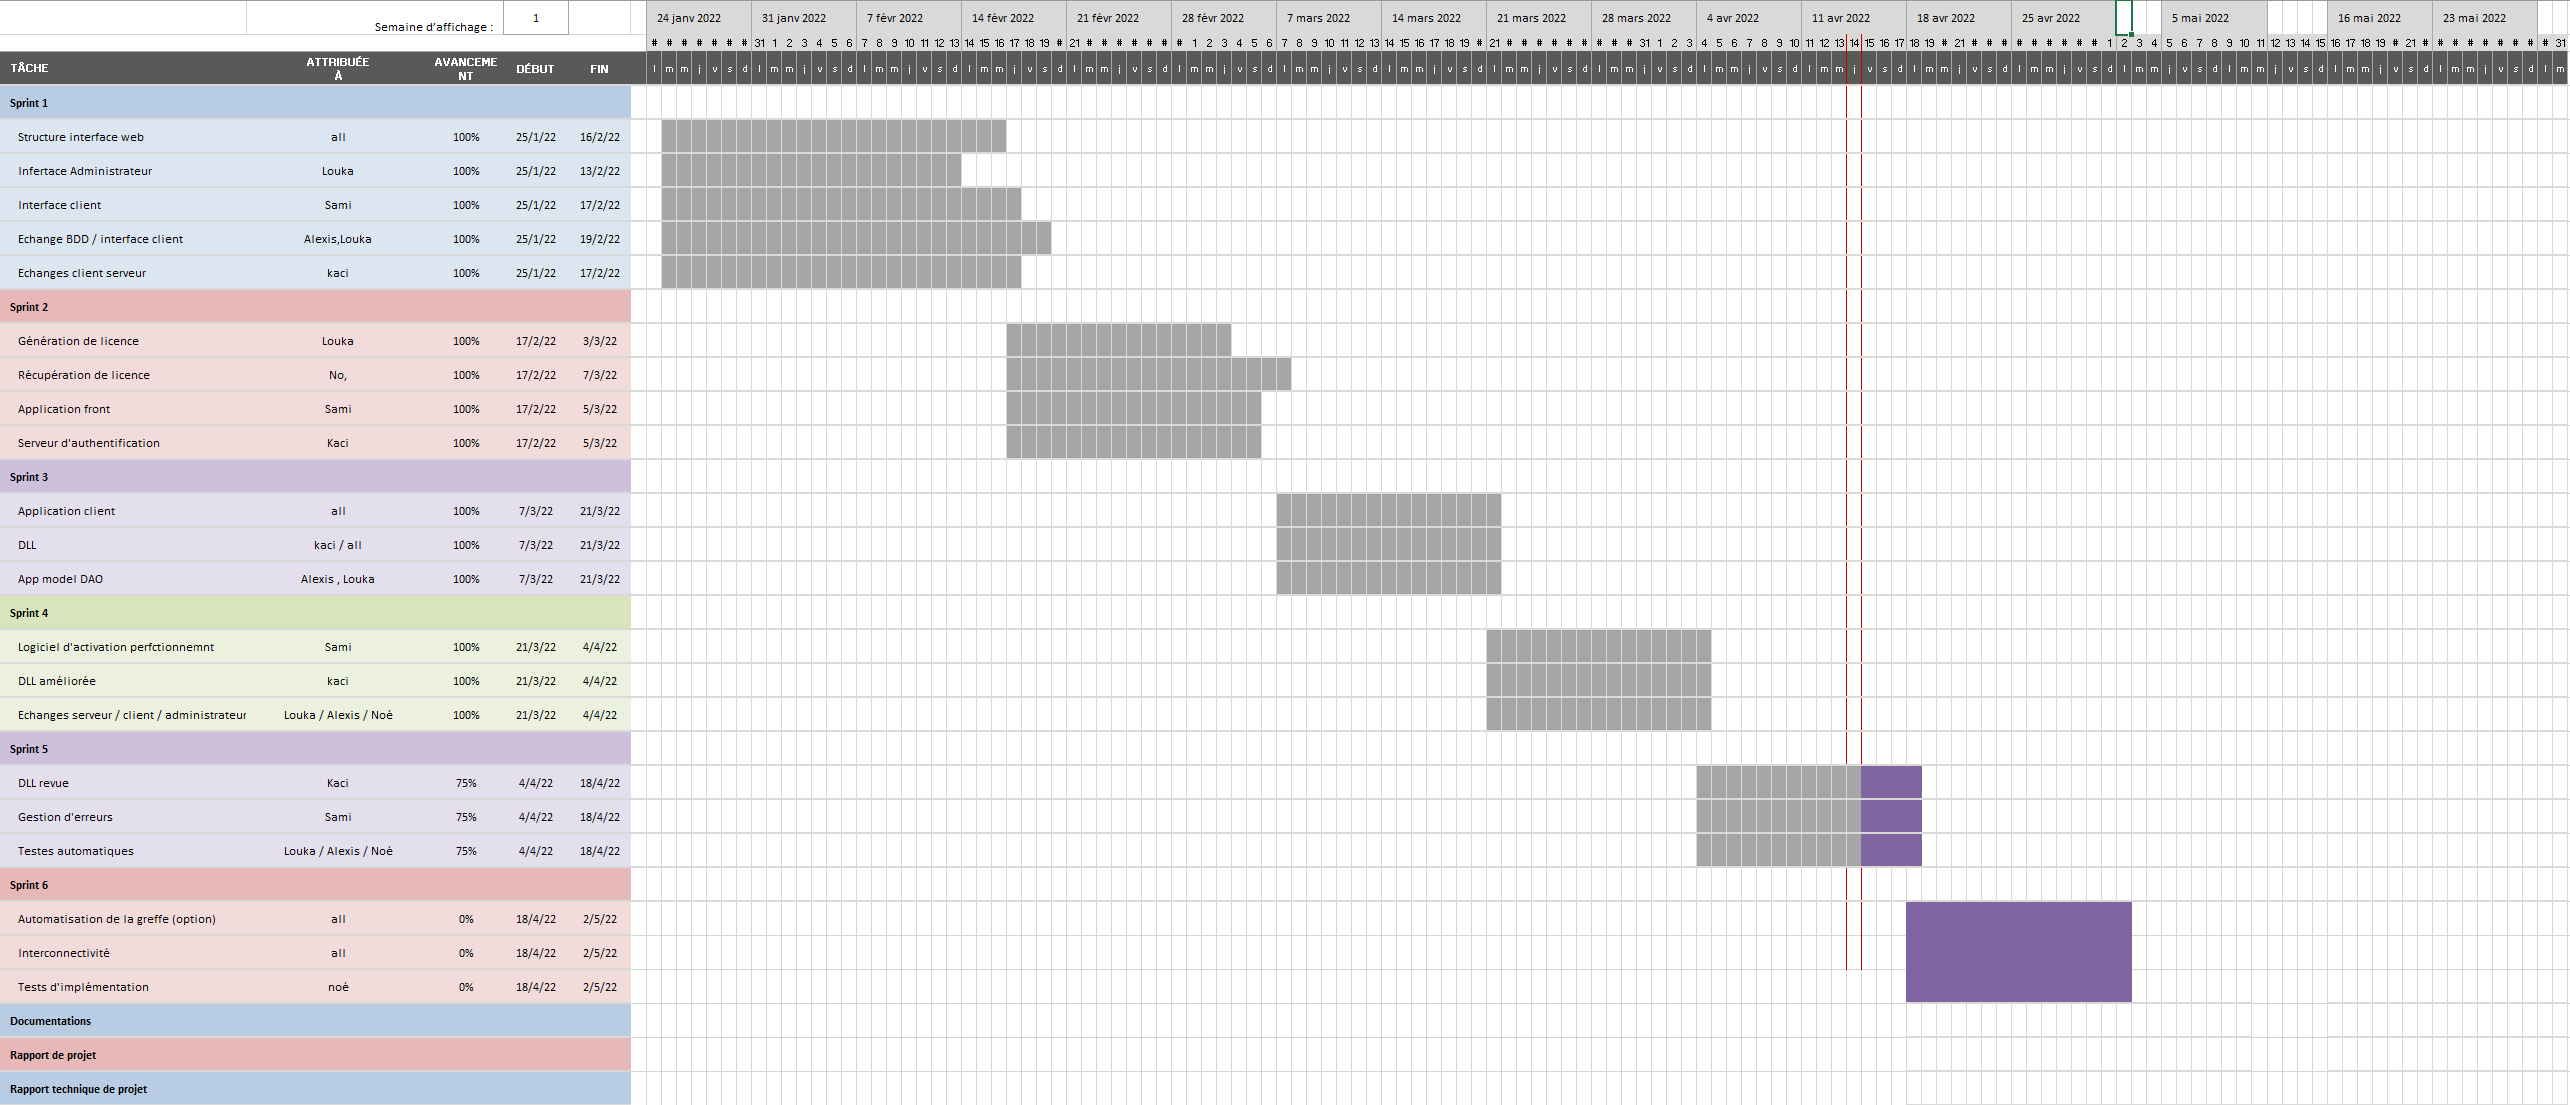
\includegraphics[width=15cm]{Gantt.png}
\end{figure}

La phase de développement du projet a donc, si nous nous referons aux anciennes estimations, suivis son cours.\newline

Celle-ci s'est donc découpé en phase de sprint de 2 semaines chacunes. Chaque sprint se décomposé de la maniere suivante :  

\begin{itemize}
	\item 1 - Réunion de debut de sprint avec l'equipe pour faire une estimation de temps de taches définies ainsi que pour les attribuer.
	\item 2 - Réunions journaliere pour faire le points sur les avancés et les bloquages.
\end{itemize}

\chapter{Implémentation}

\section{Licence}

\section{Outils de gestion}

\section{DLL}

\chapter{Système}

\section{Machine virtuelle d'authentification}

\section{Machine virtuelle web}

\chapter{Problèmes rencontrés}

\chapter{Amélioration possible}

\section{Injection de code}

\section{Invalidation de date}

\chapter{Conclusion}
\label{chapter:bilan}

